

\section{Background}

Proxy servers help communication between two entities on a network. They often act as intermediaries between clients and content-delivering servers. They help optimize and add structure to networks and distributed systems. The latency incurred from downloading content directly from target servers is fast becoming a limiting factor on ‘internet speeds’. With sharp upward trends in the number of devices connected to the internet, this has forced cell-phone providers, ISPs and even large local area networks to use these servers to optimize both networks and content delivery. As a result, end users consciously and unconsciously end up using several proxies a day. While these proxies have sophisticated caching and compression mechanisms, they are stand-alone programs that do not do the most they can to share information about users and the data they are caching.

\begin{figure}[H] \centering
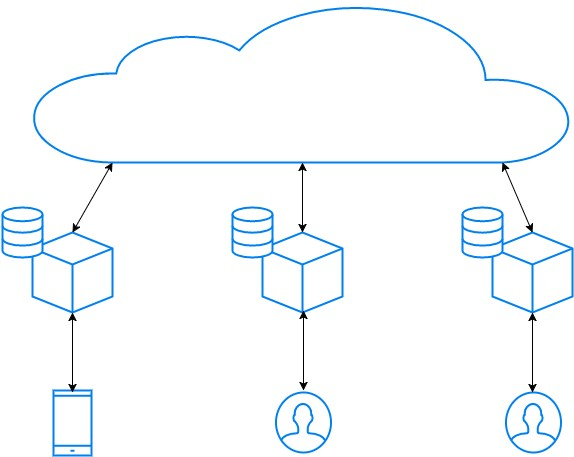
\includegraphics[width=\textwidth]{TraditionalArch}
\caption{Traditional Client-Proxy Architecture}
\end{figure}


In Figure 1 we can see a simple representation of the traditional role proxies have. Users connect to proxy servers as intermediaries to their connection to a network, such as the internet. Each of these proxies traditionally has its own disk and RAM cache. It is also possible to utilize these proxies as a distributed network with a shared cache represented by \lq joining \rq each of the disk caches into a unified cache. However, this cache still only incorporates the basic levels of disk and RAM storage and there is potentially significant overhead in communicating between proxies to locate content that may be on a different physical machine than the one handling the request and serving the content.



\section{Flying Squid}

\subsection{Apache Traffic Server}

Apache Traffic Server (ATS) is a high-performance open-source proxy that was built by Inktomi and Yahoo!. It is modular in nature, and is known for its efficient caching mechanisms. According to the ATS documentation, it \lq \lq is designed to improve content delivery for enterprises, Internet service providers (ISPs), backbone providers, and large intranets by maximizing existing and available bandwidth \rq \rq \cite{ATS}.

Flying Squid is an Apache Traffic Server augmentation that can provide a distributed, cloud based cache localized at the edge of the network. The system utilizes custom caching techniques and protocols to reduce uneccesary bandwidth use. Thus, it provides faster data delivery than content providers by themselves. 


Flying Squid aims to be a truly web-based personal proxy, with shared cloud based caches and value-based storage and transfer protocols. By improving content delivery speed and reducing client data usage, the proxy is especially useful to mobile users and those with spotty network connectivity.